\label {fs-experiments}

\begin{figure}
\centering
\small
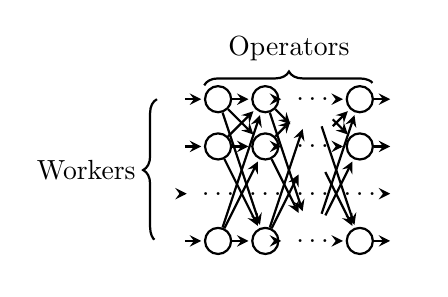
\begin{tikzpicture}[%
  ->, 
  >=stealth,
  shorten >=1pt,
  node distance=0.6cm,
  thick,
  every state/.style={%
  fill=white,
  draw=black,
  text=black
  }   
  ]
    \node[draw, circle] (I_1) [draw=none] {};
    \node[draw, circle] (I_2) [below of=I_1,draw=none] {};
    \node[draw, circle] (I_dots) [below of=I_2,draw=none] {};
    \node[draw, circle] (I_3) [below of=I_dots,draw=none] {};

    \node[draw, circle] (A_1) [right of=I_1] {};
    \node[draw, circle] (A_2) [below of=A_1] {};
    \node[draw, circle] (A_dots) [below of=A_2,draw=none] {$\ldots$};
    \node[draw, circle] (A_3) [below of=A_dots] {};

    \node[draw, circle] (B_1) [right of=A_1] {};
    \node[draw, circle] (B_2) [below of=B_1] {};
    \node[draw, circle] (B_dots) [below of=B_2,draw=none] {$\ldots$};
    \node[draw, circle] (B_3) [below of=B_dots] {};

    \node[draw, circle] (Dots_1) [right of=B_1,draw=none] {$\ldots$};
    \node[draw, circle] (Dots_2) [below of=Dots_1,draw=none] {$\ldots$};
    \node[draw, circle] (Dots_dots) [below of=Dots_2,draw=none] {$\ldots$};
    \node[draw, circle] (Dots_3) [below of=Dots_dots,draw=none] {$\ldots$};

    \node[draw, circle] (Z_1) [right of=Dots_1] {};
    \node[draw, circle] (Z_2) [below of=Z_1] {};
    \node[draw, circle] (Z_dots) [below of=Z_2,draw=none] {$\ldots$};
    \node[draw, circle] (Z_3) [below of=Z_dots] {};

    \node[draw, circle] (O_1) [right of=Z_1,draw=none] {};
    \node[draw, circle] (O_2) [below of=O_1,draw=none] {};
    \node[draw, circle] (O_dots) [below of=O_2,draw=none] {};
    \node[draw, circle] (O_3) [below of=O_dots,draw=none] {};

    \path
          (I_1) edge (A_1)
          (I_2) edge (A_2)
          (I_dots) edge (A_dots)
          (I_3) edge (A_3)
          (A_1) edge (B_1)
          (A_1) edge (B_2)
          (A_1) edge (B_3)
          (A_2) edge (B_1)
          (A_2) edge (B_2)
          (A_2) edge (B_3)
          (A_3) edge (B_1)
          (A_3) edge (B_2)
          (A_3) edge (B_3)
          (B_1) edge (Dots_1)
          (B_1) edge (Dots_2)
          (B_1) edge (Dots_3)
          (B_2) edge (Dots_1)
          (B_2) edge (Dots_2)
          (B_2) edge (Dots_3)
          (B_3) edge (Dots_1)
          (B_3) edge (Dots_2)
          (B_3) edge (Dots_3)
          (Dots_1) edge (Z_1)
          (Dots_1) edge (Z_2)
          (Dots_1) edge (Z_3)
          (Dots_2) edge (Z_1)
          (Dots_2) edge (Z_2)
          (Dots_2) edge (Z_3)
          (Dots_3) edge (Z_1)
          (Dots_3) edge (Z_2)
          (Dots_3) edge (Z_3)
          (Z_1) edge (O_1)
          (Z_2) edge (O_2)
          (Z_dots) edge (O_dots)
          (Z_3) edge (O_3)
          ;
      \draw[-,thick,decorate,decoration={brace,amplitude=5pt,mirror}]
            ([xshift=-5pt]I_1.center) -- ([xshift=-5pt]I_3.center) node[midway, left=4pt] {Workers};
      \draw[-,thick,decorate,decoration={brace,amplitude=5pt}]
            ([xshift=-5pt, yshift=5pt]A_1.center) -- ([xshift=5pt, yshift=5pt]Z_1.center) node[midway, above=5pt] {Operators};
\end{tikzpicture}
\caption{Physical execution graph for experiments} 
\label{fig:physical_graph}
\end{figure}

% https://gist.github.com/faucct/032aaf6240db361d30a184b1d7bf3c8e
\begin{figure*}[t!]
    \begin{subfigure}[b]{0.30\textwidth}
            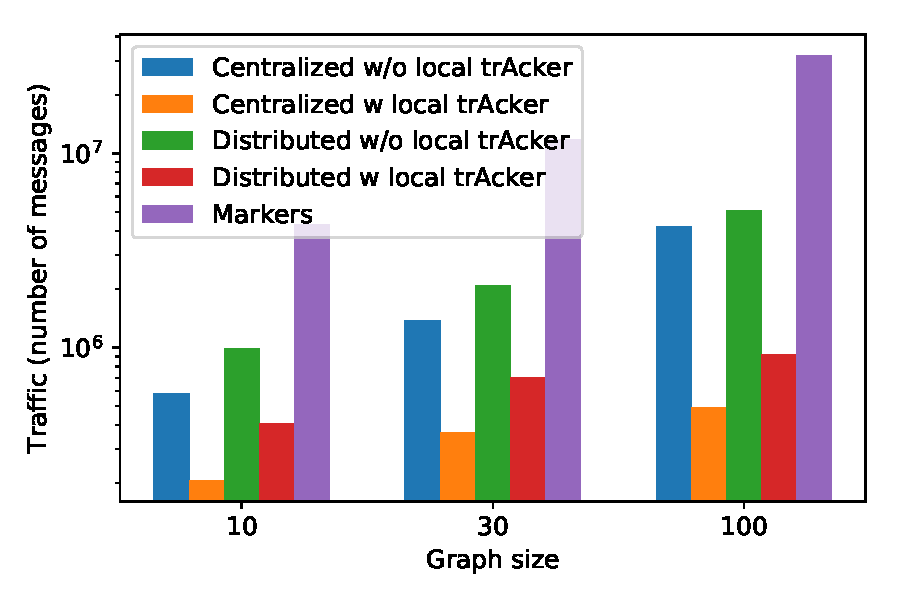
\includegraphics[width=0.99\textwidth]{pics/traffic_by_graph_size_bars.pdf}
            \caption{Traffic by graph size}
            \label{traffic_graph}
    \end{subfigure}
    \hspace{5mm}
    \begin{subfigure}[b]{0.30\textwidth}
            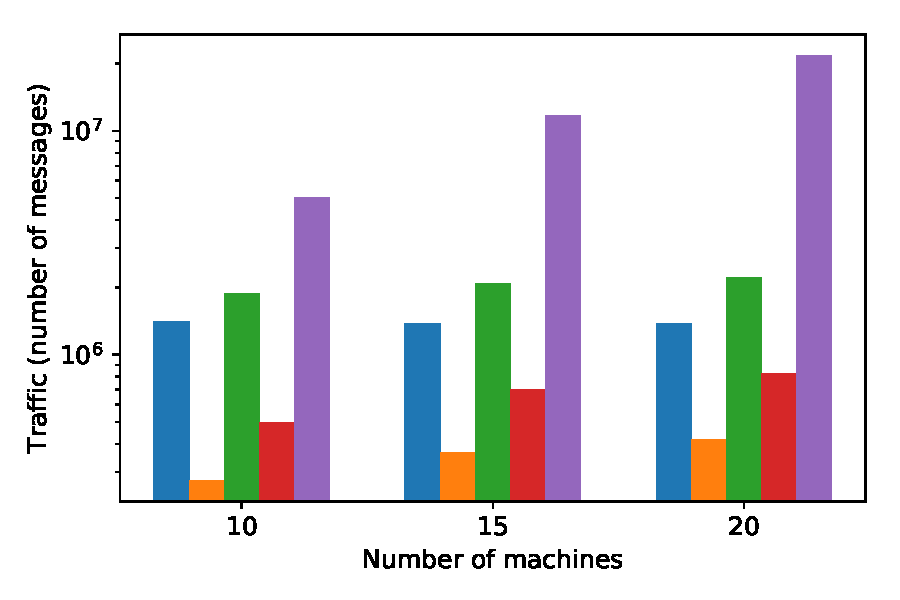
\includegraphics[width=0.99\textwidth]{pics/traffic_by_number_of_machines_bars.pdf}
            \caption{Traffic by number of virtual machines}
            \label{traffic_machines}
    \end{subfigure}
    \hspace{5mm}
    \begin{subfigure}[b]{0.30\textwidth}
            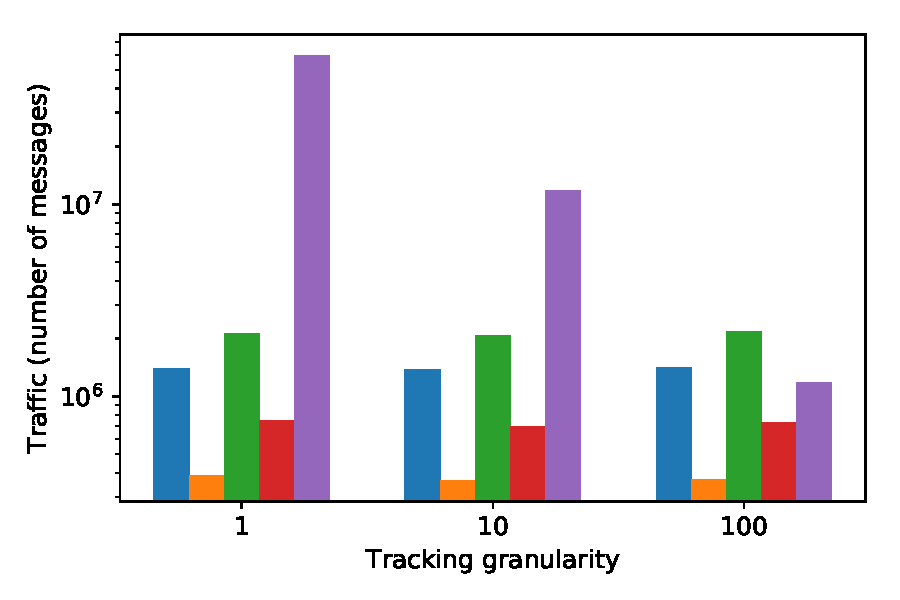
\includegraphics[width=0.99\textwidth]{pics/traffic_by_tracking_frequency_bars.pdf}
            \caption{Traffic by tracking frequency}
            \label{traffic_granularity}
    \end{subfigure}
    \caption{Service network traffic of punctuations approach and various \tracker\ setups}
    \label{traffic_plots}
\end{figure*}
In previous sections of the paper, we put several statements out: \tracker\ framework provides low service traffic, low latency between the actual substream termination and termination event receiving, and SPE throughput does not depend on the substream size. In the experimental part of the paper, we will demonstrate these properties on synthetic and real-world examples. 

As a baseline approach, we utilize the punctuations-based method employed in many state-of-the-art stream processing systems such as Flink~\cite{Carbone:2017:SMA:3137765.3137777}, Storm~\cite{apache:storm:state}, Heron~\cite{Kulkarni:2015:THS:2723372.2742788}, IBM Streams~\cite{jacques2016consistent}, etc. To the best of our knowledge, the punctuation framework is the only existing general-purpose substream management technique.

Our goal is to explore how the change of the tracking mechanism affects the behavior of an SPE. We implemented both methods on top of an open-source distributed streaming engine called \FlameStream. Functionality and use-cases of this SPE are similar to state-of-the-art stream processing systems (Flink, Storm, etc.). None of the system-specific features were exploited during the implementation of substream management methods. All experiments are performed on virtual machines with a dual-core CPU and 4 GB RAM from one of the major cloud providers. 

In the next sections, we will explore our system in four experimental setups:
% \begin{description}
    
    \noindent \textbf{Service traffic:} the last setup aims to demonstrate the asymptotic behavior of competitive approaches. We show that our theoretical estimation meets practical measurements.
    
    \noindent \textbf{Notification latency:} we explore a delay between a moment when a substream ends and the reception of the termination event for this substream. We compare notification latency of the \tracker\ and punctuations approaches for both synthetic and real-world workloads in soft and firm bound cases.
    
    \noindent \textbf{Maximum SPE throughput:} we study the influence of the notification mechanism on the maximum throughput of the system using the synthetic workload. This experiment shows an overhead induced by a substream management mechanism on regular data processing.
    
    \noindent \textbf{Substream management for cyclic graphs:} \tracker\ framework supports substream management for cyclic dataflows. In this setup, we demonstrate the benefits of this approach for a novel problem setup: state smart caching.

% \end{description}

In our study, we use a common synthetic workload shown in Fig.~\ref{fig:physical_graph}. All vertices pass an input element to the next operation. On each step, items are re-partitioned (round-robin). This shape of the physical execution graph allows us to measure the properties of the system with the growth of key switches in a workload. This setup has no computational overhead while covering many realistic scenarios. Graphs with few vertices (under 30) may fit almost any acyclic streaming pipeline~\cite{akidau2018streaming}. Longer instances of this workload correspond to flattened iterative dataflows such as PageRank or Connected Components~\cite{Murray:2013:NTD:2517349.2522738, xu2016efficient}. We reference this synthetic workload as RR-$N$, where $N$ is the number of steps.

To compare tracking mechanisms, we have to implement them on top of a single SPE. Otherwise, the performance could be affected by inequalities in serialization, network protocols, etc.  The difficulty here is that the tracking mechanism is usually a core part of SPE, and the implementation is often optimized for it. 

We implemented both punctuations and \tracker\ techniques on top of \FlameStream~\cite{we2018beyondmr}. It is an open-source Java-based SPE that allows tracking mechanism customization by its design. In~\cite{we2018adbis}, authors demonstrated that the performance of the \FlameStream\ is comparable to state-of-the-art SPE Flink.

\subsection{Service traffic}
\label{exp_network_traffic}
In the theoretical part of the paper, we put a statement that the service traffic of the \tracker\ grows linearly with the number of processes and granularity of the tracking. In this section, we prove this statement in practice. 

We can measure the extra load provided by tracking mechanisms in a number of service messages sent over the network. In \tracker, there are several types of these messages: SND and RCV reports, NEOSS, and logical clock vectors in the distributed setup. In the baseline approach, all service messages are punctuations.

Figure~\ref{traffic_plots} demonstrates the dependency between service network messages and the size of the logical graph, the number of computational nodes, and the granularity of tracking. The extra service traffic is generated by $50K$ input elements sent with 100 items per second arrival rate. 

As shown in Figure~\ref{traffic_graph}, service traffic for punctuations linearly depends on the dataflow size because each new logical vertex adds network broadcasts of punctuations on a physical level. Dependency from the number of computational nodes is quadratic \footnote{At first glance, the dependency may seem linear, but please note that the X-axis covers range from 10 to 20, and the Y-axis is log-scaled} due to the need to broadcast punctuations to each node after each operator, as it is demonstrated in Figure~\ref{traffic_machines}. 

Figure~\ref{traffic_granularity} indicates that the number of sent service messages for punctuations also directly depends on the tracking granularity. For example, the system should broadcast punctuations after each streaming element in every operator to implement tracking of individual items. 

In the case of \tracker, service traffic depends on the logical graph size and the number of machines because their product forms the number of processes. The growth has a linear trend but can be significantly reduced with the local \tracker\ optimization. Distributed \tracker\ without optimizations provides ~10x less service than punctuations traffic for a graph with 10 vertices and ~30x decrease for a graph with 100 vertices. Regarding the number of machines, the difference is ~10x for 10 nodes and ~30x for 20 nodes. Besides, local \tracker\ optimization allows the system to reduce traffic up to 5 times compared to the straightforward implementation of the distributed \tracker.

\subsection{Microbenchmarks: notification latency}
% https://gist.github.com/faucct/032aaf6240db361d30a184b1d7bf3c8e
\begin{figure*}[t!]
    \begin{subfigure}[b]{0.30\textwidth}
            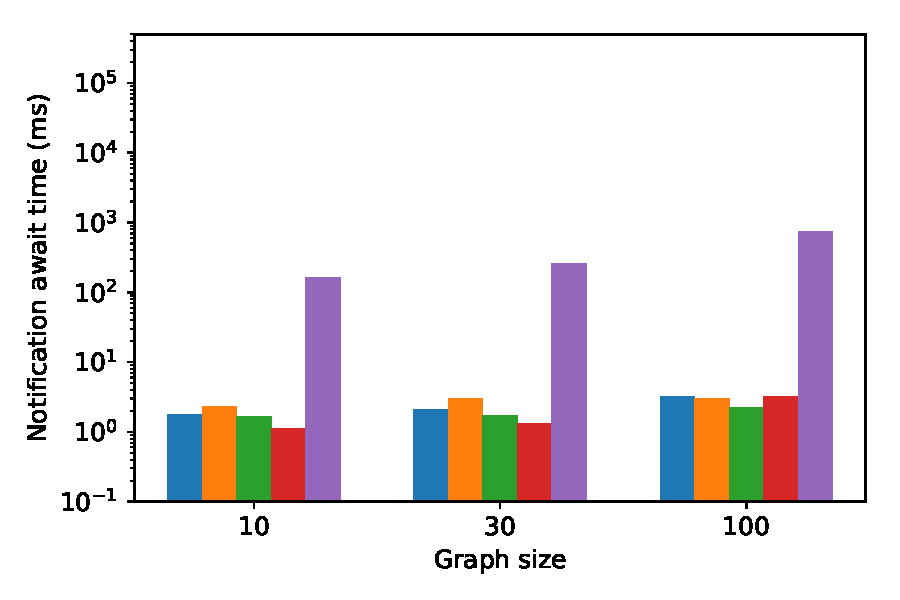
\includegraphics[width=0.99\textwidth]{pics/notification_await_time_by_graph_size_bars.pdf}
            \caption{Notification latency by graph size}
            \label{notification_graph}
    \end{subfigure}
    \hspace{5mm}
    \begin{subfigure}[b]{0.30\textwidth}
            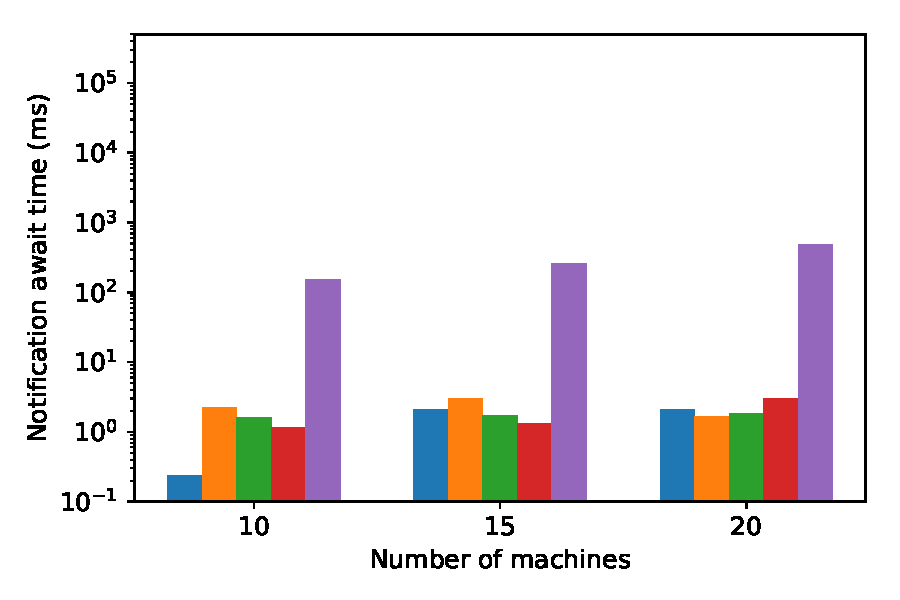
\includegraphics[width=0.99\textwidth]{pics/notification_await_time_by_number_of_machines_bars.pdf}
            \caption{Notification latency by VMs number}
            \label{notification_machines}
    \end{subfigure}
    \hspace{5mm}
    \begin{subfigure}[b]{0.30\textwidth}
            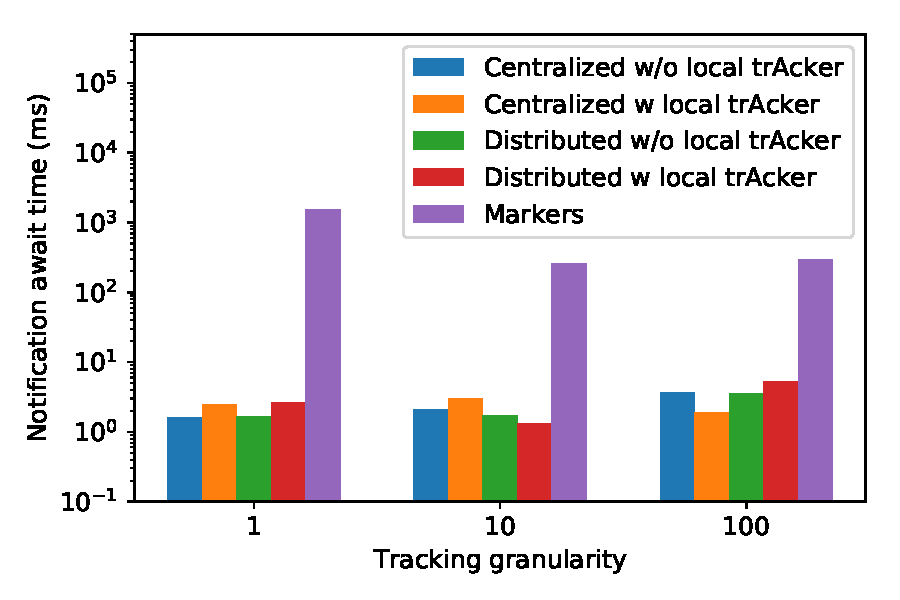
\includegraphics[width=0.99\textwidth]{pics/notification_await_time_by_tracking_frequency_bars.pdf}
            \caption{Notification latency by granularity}
            \label{notification_granularity}
    \end{subfigure}
    \caption{Notification latency}
    \label{notification_latency}
\end{figure*}

One of the key performance metrics is the latency of notifications: a delay between a moment when a substream ends and the reception of the termination event. This time is added to any operation triggered by termination events~\cite{Carbone:2017:SMA:3137765.3137777, we2018adbis}. For example, Flink finishes its state snapshotting protocol for the epoch (set of input elements) and delivers corresponding output elements to data consumers only after receiving a notification that the whole epoch is completed. We examine end-to-end latency in the next section.

There are two experiments in this setting. We will first measure notification latency in lightweight synthetic workload to compare the absolute cost of different substream management algorithms. The main risk that comes from the introduction of a centralized agent is the lack of scalability of this agent, and in the second experiment, we will study the performance of the distributed tracking agent.

\subsubsection{Absolute notification latency}
\label{absolute-latency}

In this experiment, we measure the notification latency as an interval duration between a promise from the data source that it will never generate substream elements and the reception of the termination event for this substream. As an experimental workload, we use synthetic workload RR-$N$. We investigate the dependency between the notification latency and cluster sizes, the length $N$ of the workload, and the granularity of tracking (number of elements within a substream). Figure~\ref{notification_latency} shows the results of the experiment. 

The notification latency of a punctuations-based technique depends on the graph and cluster sizes and the granularity of tracking as figures~\ref{notification_graph},\ref{notification_machines}, and~\ref{notification_granularity} indicate. These results are in-line with the overhead induced by punctuations shown in Section~\ref{fs-acker-punctuations}. Notification latency of \tracker\ slightly fluctuates but does not directly depend on the investigated parameters. One can also note that local \tracker\ optimization, as well as distributed version, does not induce heavy overhead on the latency.

Such a significant difference in latency between the punctuations and \tracker\ is explained by the fact that each operator in a dataflow must wait for punctuations from all partitions of the previous operator to send it further. This behavior ensures that punctuations do not overtake ordinary records that guarantee the correctness of this approach.

% \subsubsection{Scalability of \tracker }
% % https://gist.github.com/faucct/546f5617b958349a125449926373b780
% \begin{figure*}[t!]
%     \begin{subfigure}[b]{0.30\textwidth}
%             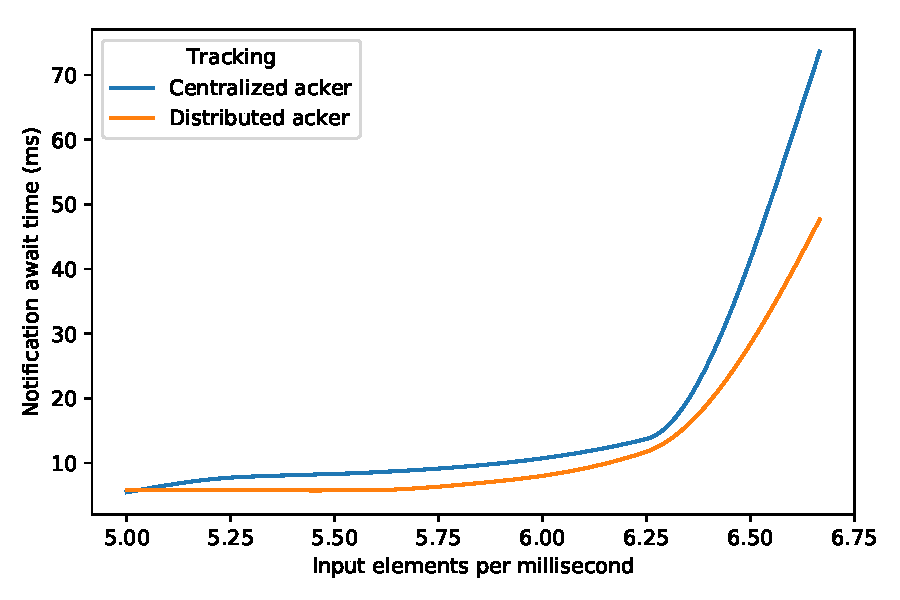
\includegraphics[width=0.99\textwidth]{pics/scalability_01x.pdf}
%             \caption{1x reports}
%             \label{1x_acks}
%     \end{subfigure}
%     \hspace{5mm}
%     \begin{subfigure}[b]{0.30\textwidth}
%             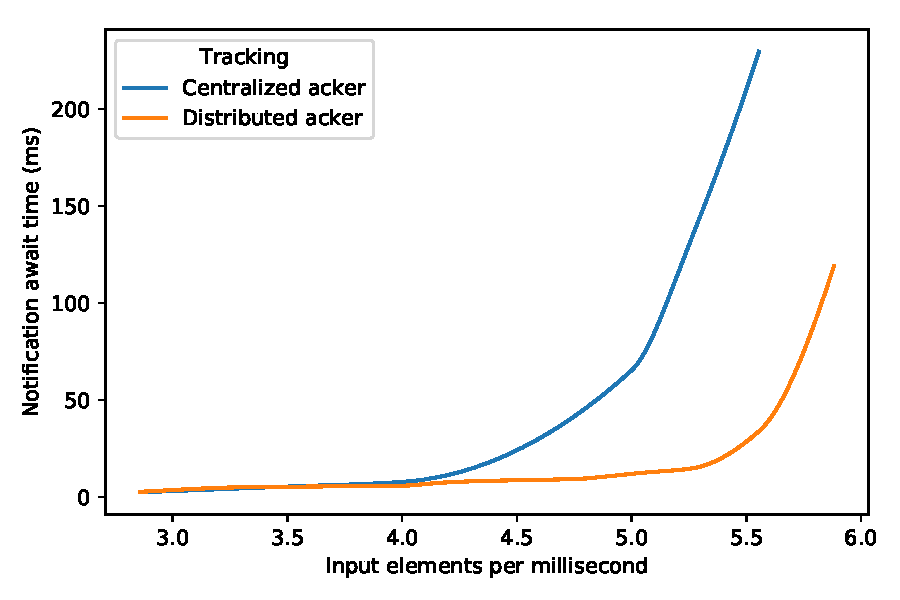
\includegraphics[width=0.99\textwidth]{pics/scalability_05x.pdf}
%             \caption{5x reports}
%             \label{5x_acks}
%     \end{subfigure}
%     \hspace{5mm}
%     \begin{subfigure}[b]{0.30\textwidth}
%             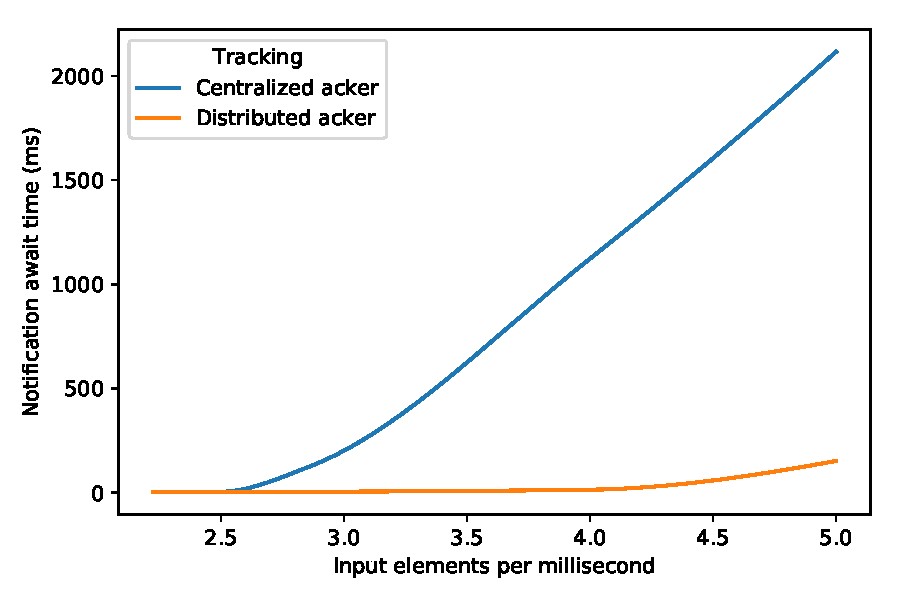
\includegraphics[width=0.99\textwidth]{pics/scalability_09x.pdf}
%             \caption{9x reports}
%             \label{9x_acks}
%     \end{subfigure}
%     \caption{\tracker\ scalability}
%     \label{notification_scalability}
% \end{figure*}
% This section demonstrates that the distributed version of the tracking agent allows the substream management mechanism to scale. We measure the median notification latency depending on the rate of input records. The rapid growth of median latency indicates agent overloading. Input rate that corresponds to the point where latency starts to grow indicates a {\em sustainable throughput} of the \tracker. 

% To simulate an additional load on the tracking agent, staying on a budget of 20 machines, we artificially increased the number of sent service messages by 5 and 9 times. We approximate the sustainable throughput by multiplying the extra service messages ratio by the obtained throughput due to the direct dependency between the input and service messages rates. This trick allows us to estimate agent throughput in the number of input data items per second rate without  SPE overloading. Figure~\ref{notification_scalability} demonstrates the results of this experiment.

% Without the extra load, distributed tracking agent provides results similar to a centralized setup, as Figure~\ref{1x_acks} indicates. Note, SPE overloading limits the throughput of the agent because it starts to delay service messages sending. Figure~\ref{5x_acks} demonstrates that with 5x simulated extra load, distributed \tracker\ can sustain $\sim 27K$ requests (items) per second input rate, while centralized provides only $\sim 20K$ RPS throughput. Figure~\ref{9x_acks} shows that with the increase of the extra load to 9x, distributed \tracker\ provides almost 2x throughput increase: $\sim 40K$ RPS against $\sim 22K$ RPS. 

% The experiments demonstrate that even the centralized tracking agent can sustain a high input rate within 20 computational nodes. Besides, the distributed version of the agent can make the tracking scalable in larger setups.

\subsection{End-to-end latency}

In the previous section we demonstrated that \tracker\ framework provides lower notification latency than the baseline. In this part, we show how this difference influence the end-to-end latency. We use real-world workloads: a window join and a state snapshot. We measure the latency of window join as a time between the last element of the window enters the system and the output of window aggregation. We also examine how substream management technique can affect the duration of taking a state snapshot. In both scenarios, end-to-end latency is directly affected by the notification latency. These experiments allow us to get the whole picture of system behavior change when we switch from one substream management to another.

\subsubsection{Window join}
For the windowed join scenario, we apply NEXMark benchmark~\cite{tucker2008nexmark} designed to inspect the performance of streaming queries. This benchmark extends the XMark benchmark~\cite{schmidt2002xmark} online auction model, where users can start auctions for items and bid on items. We accept Query 8 from the NEXMark benchmark, defined as follows: {\em Select people who have entered the system and created auctions in the last period}. This query can be implemented using windowed join of persons and auctions. We apply 10 seconds window and 500 RPS per node input rate.

% \begin{figure}[htbp]
%   \centering
%   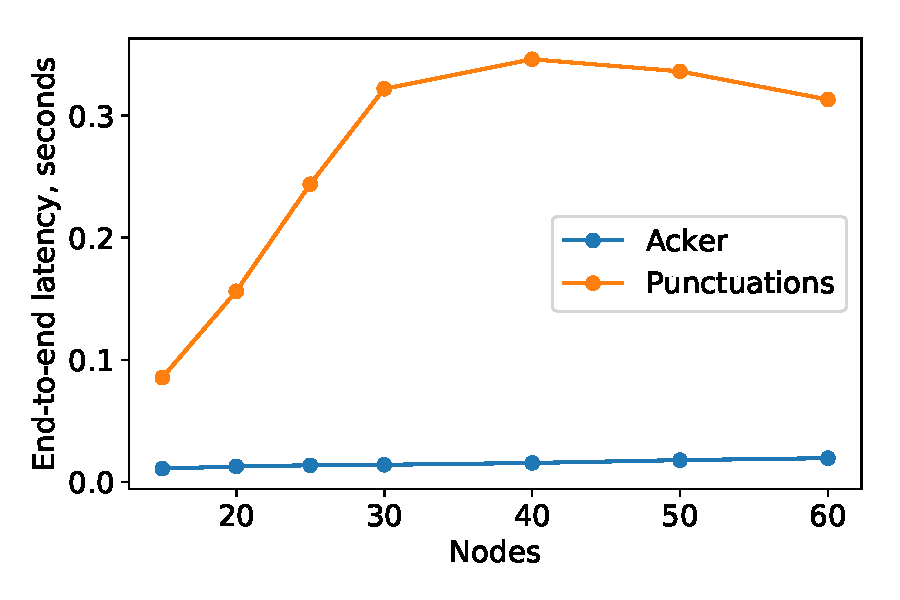
\includegraphics[width=0.40\textwidth]{pics/nexmark.pdf}
%   \caption{Notification latency for Nexmark window join scenario}
%   \label{fig:nexmark}
% \end{figure}

Figure~\ref{fig:nexmark} illustrates the results. The end-to-end latency (a time between the last element of the window enters the system and the output of window aggregation) within \tracker\ is under 20ms for all setups, while within punctuations latency grows up to ~300ms on 30 nodes. After that it fluctuates slightly. This behavior can be explained by the fact that process waits for punctuations from all channels to produce query result. However, with the growth of machines number, the probability that some node delays punctuation increases. After some limit (30 nodes in our case), many nodes start to delay punctuations, so the latency achieves its maximum. 

\subsubsection{State snapshooting}
\begin{figure*}[t!]
    \begin{subfigure}[b]{0.30\textwidth}
            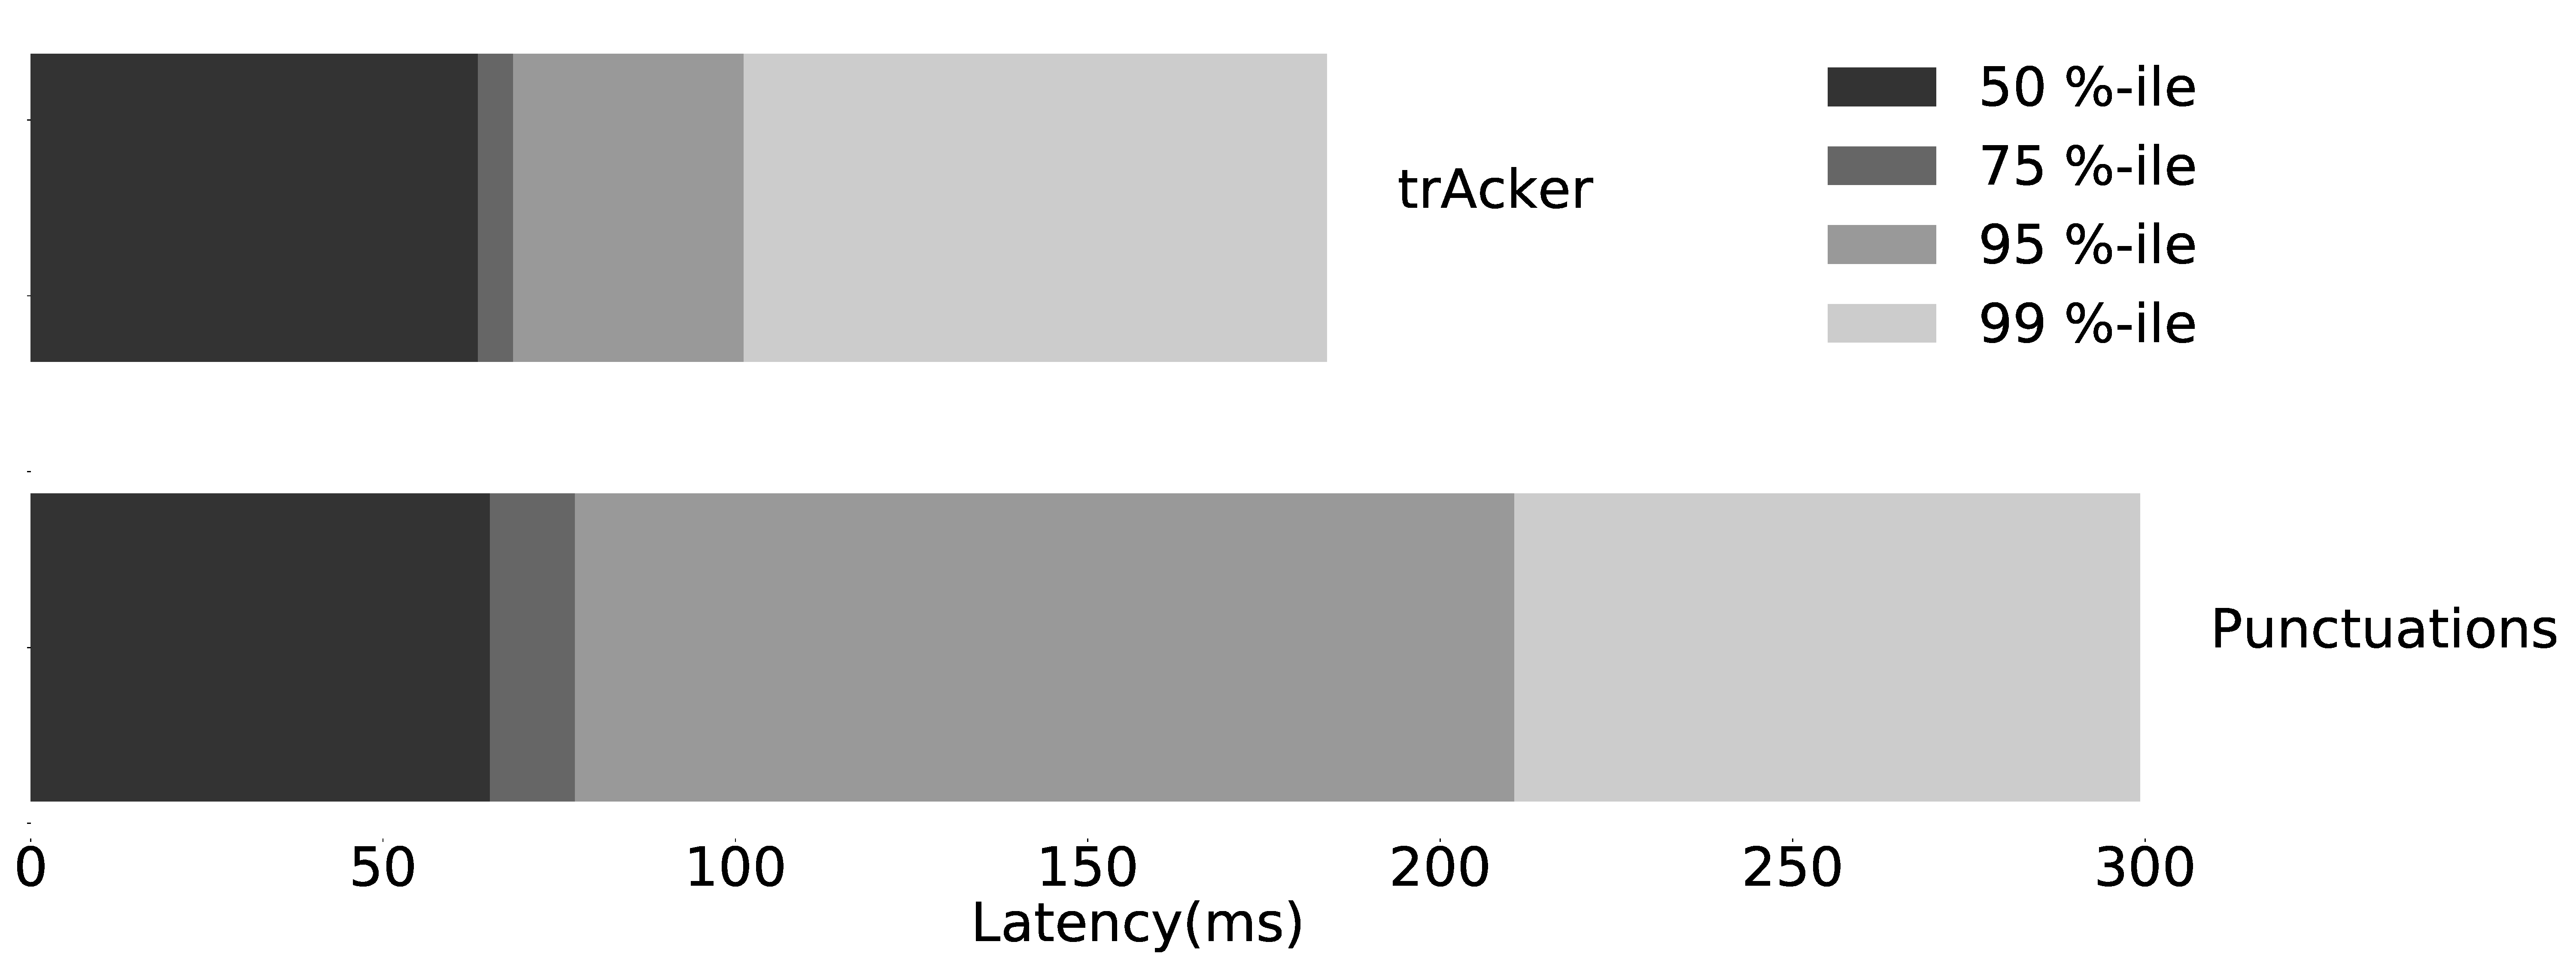
\includegraphics[width=0.99\textwidth]{pics/buffering_latencies_barh_100.pdf}
            \caption{100 ms snapshot duration}
            \label{100ms_snapshot}
    \end{subfigure}
    \hspace{5mm}
    \begin{subfigure}[b]{0.30\textwidth}
            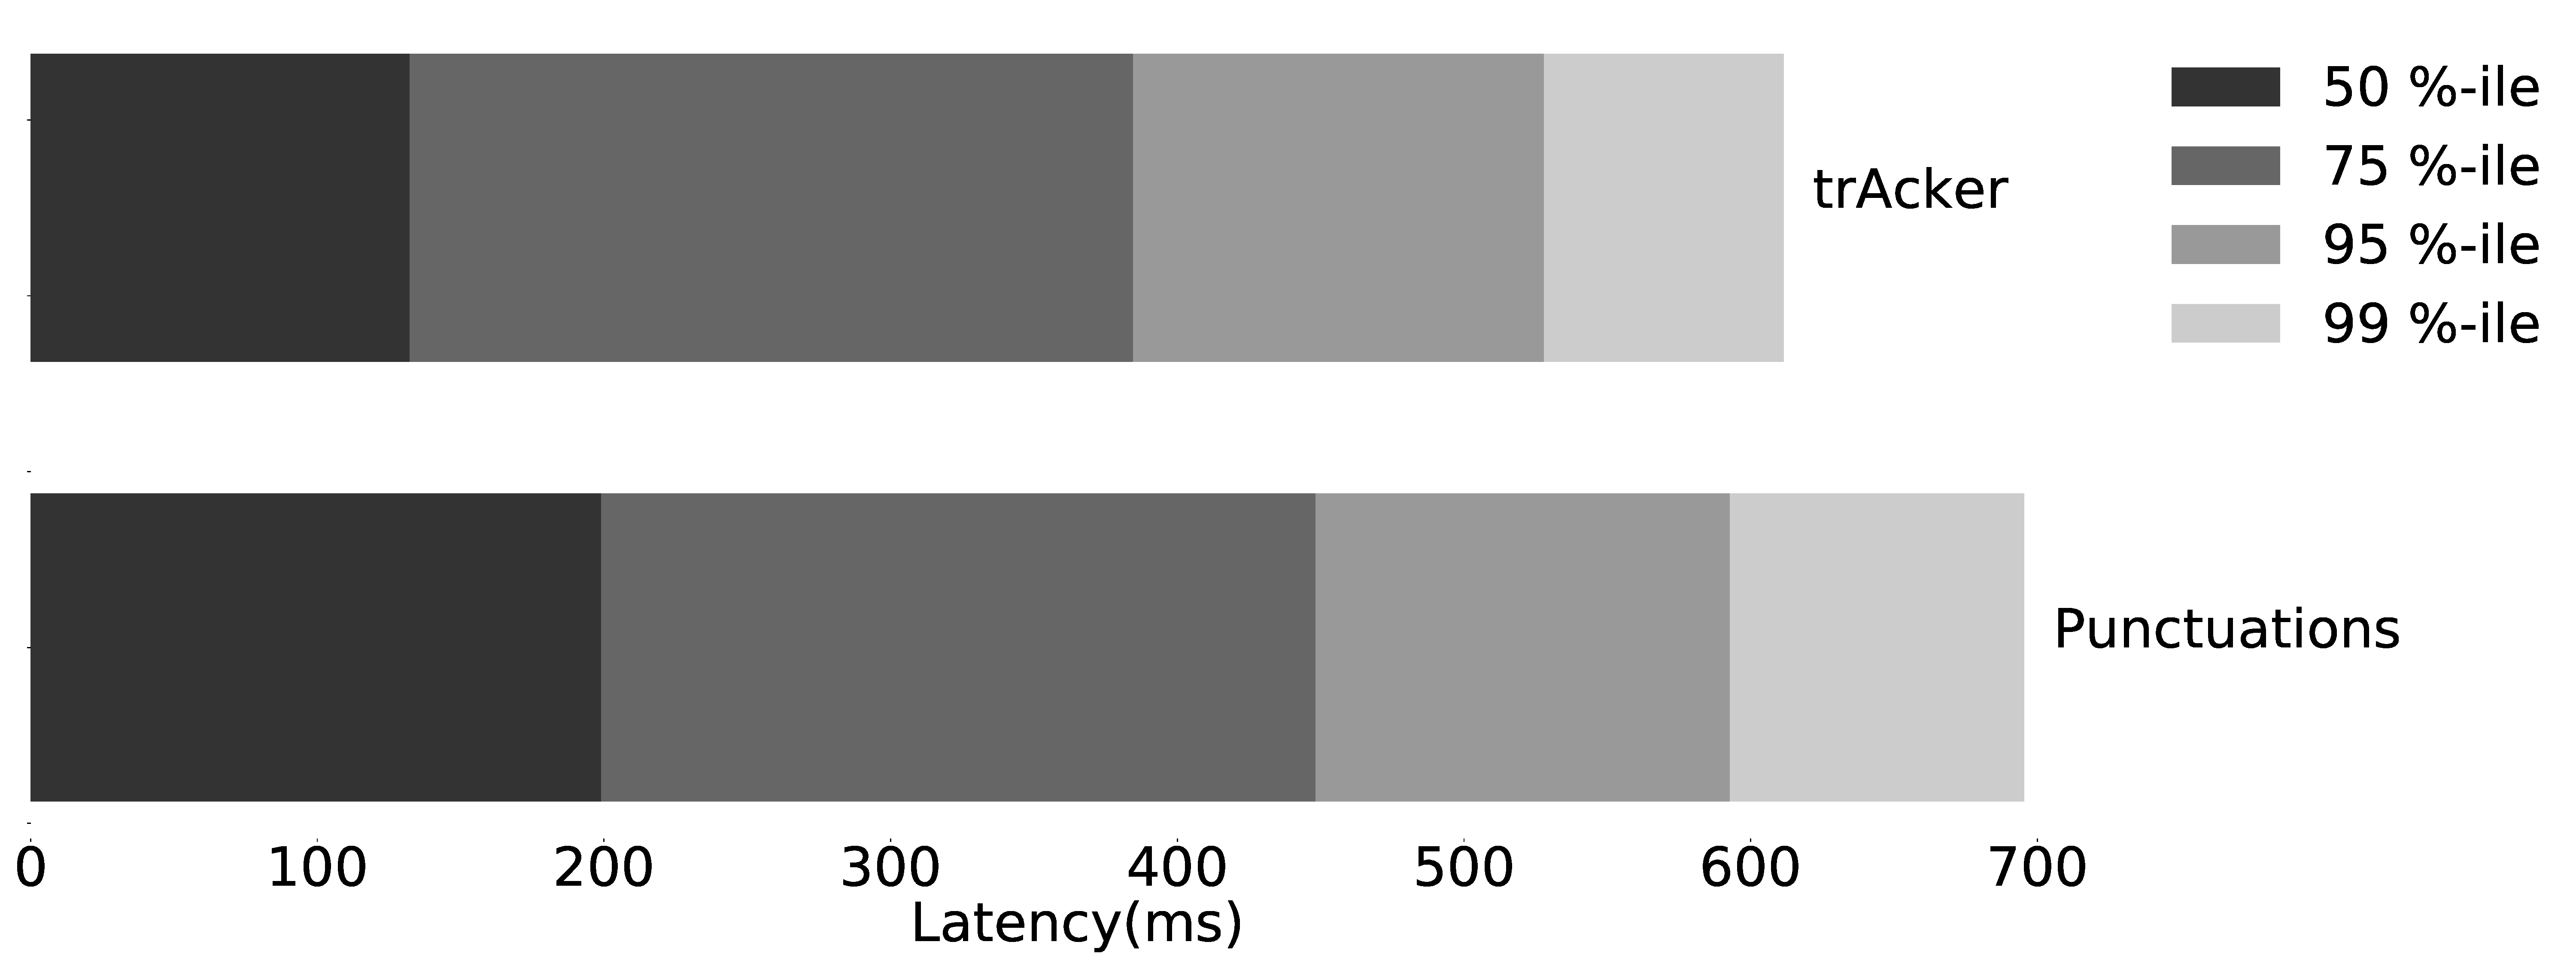
\includegraphics[width=0.99\textwidth]{pics/buffering_latencies_barh_500.pdf}
            \caption{500 ms snapshot duration}
            \label{500ms_snapshot}
    \end{subfigure}
    \hspace{5mm}
    \begin{subfigure}[b]{0.30\textwidth}
            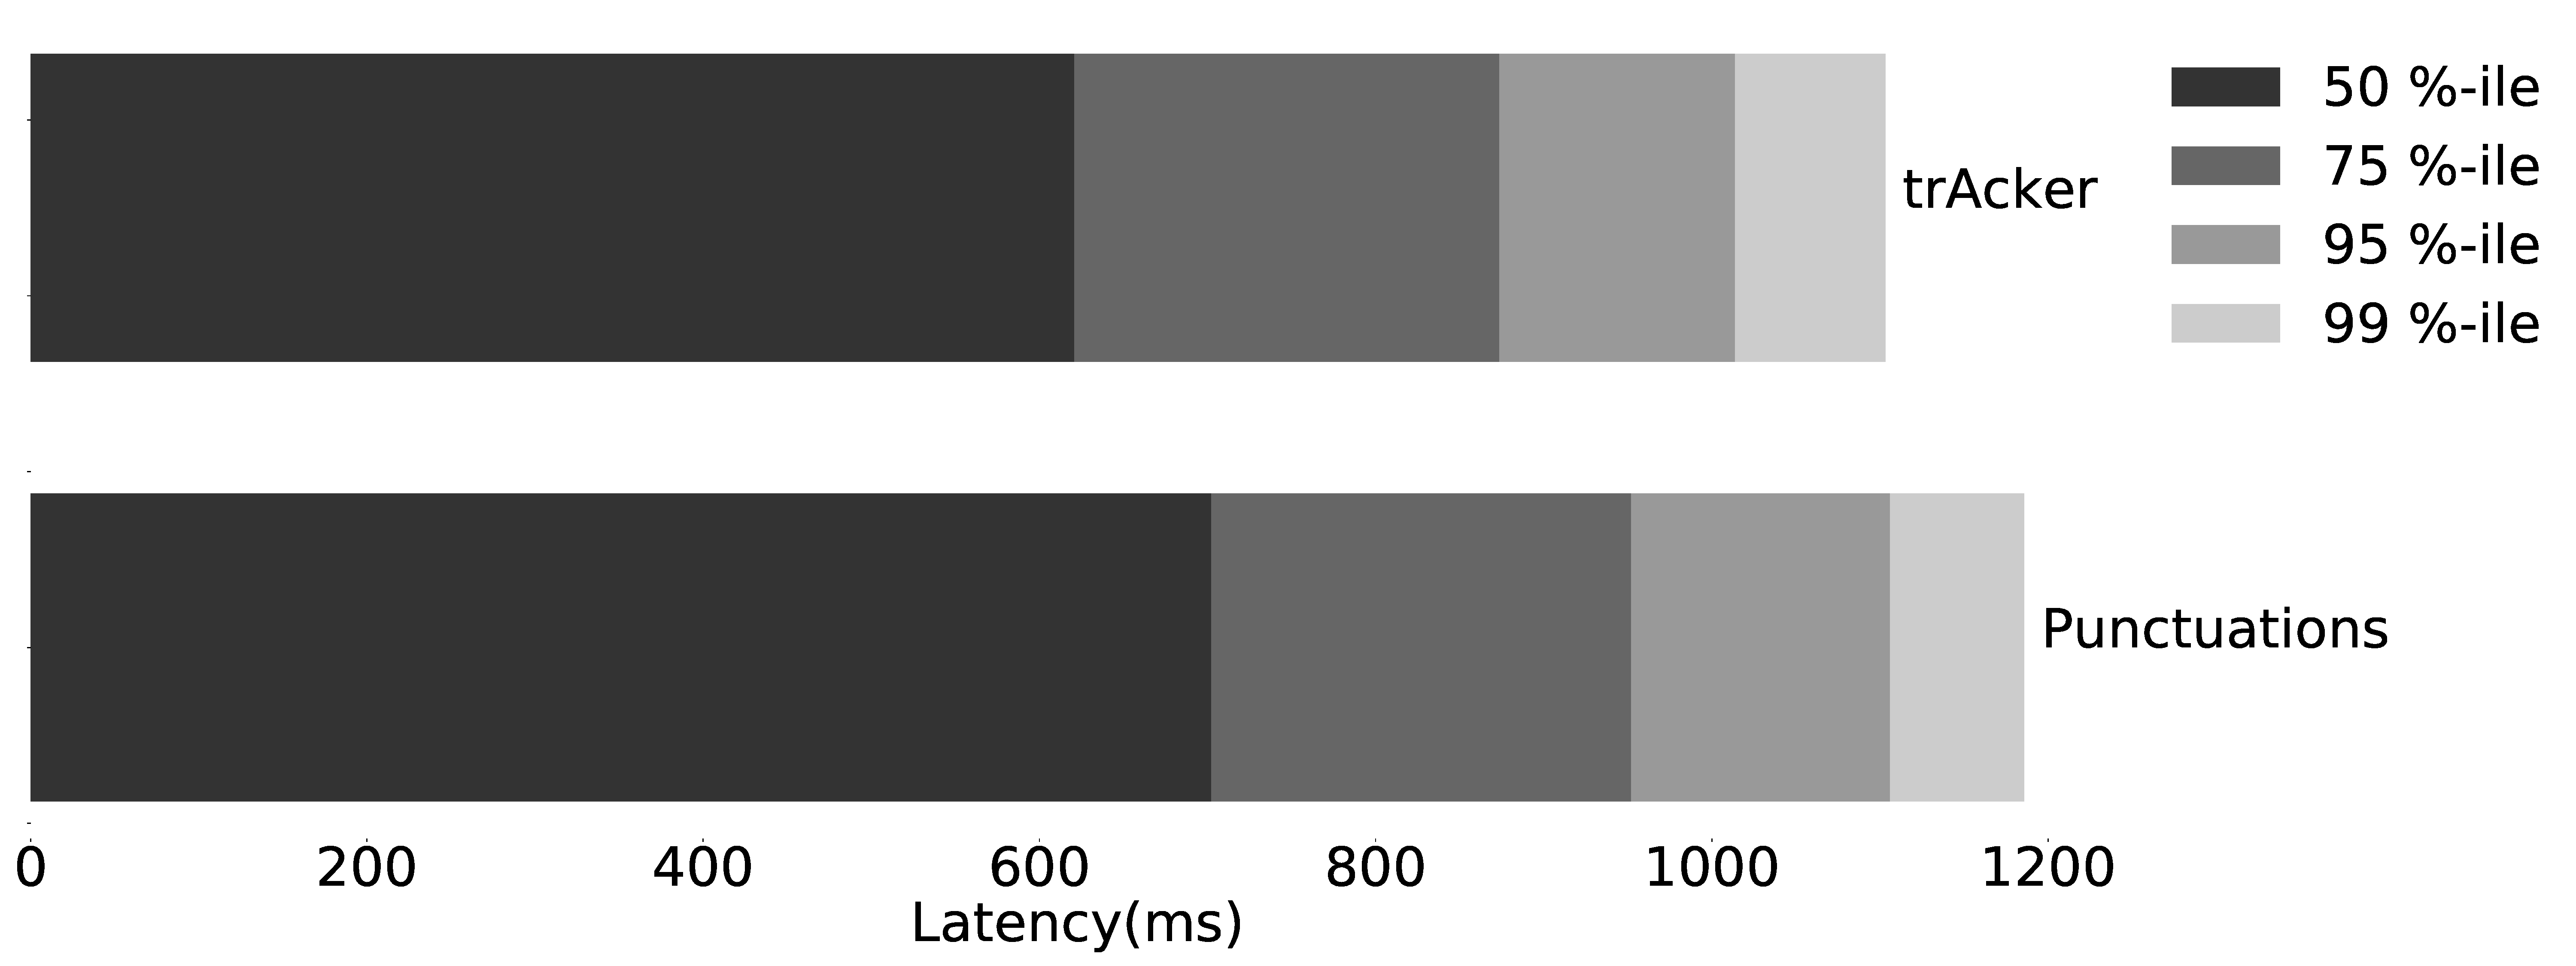
\includegraphics[width=0.99\textwidth]{pics/buffering_latencies_barh_1000.pdf}
            \caption{1000 ms snapshot duration}
            \label{1000ms_snapshot}
    \end{subfigure}
    \caption{SPE latency spikes during state snapshotting}
    \label{snapshot_spikes}
\end{figure*}

\begin{figure*}[t!]
    \begin{subfigure}[b]{0.30\textwidth}
            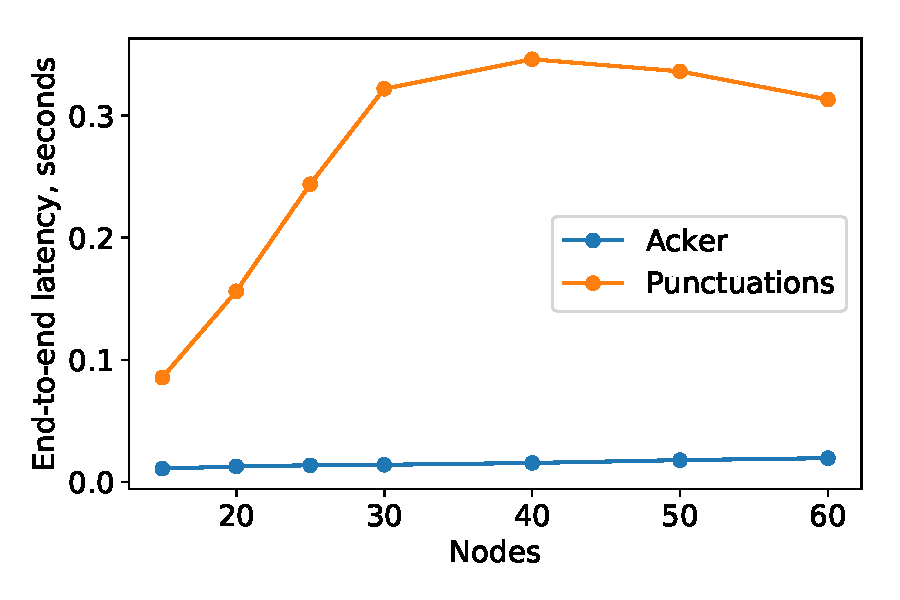
\includegraphics[width=0.99\textwidth]{pics/nexmark.pdf}
            \caption{Nexmark window join scenario}
            \label{fig:nexmark}
    \end{subfigure}
    \hspace{5mm}
    \begin{subfigure}[b]{0.30\textwidth}
            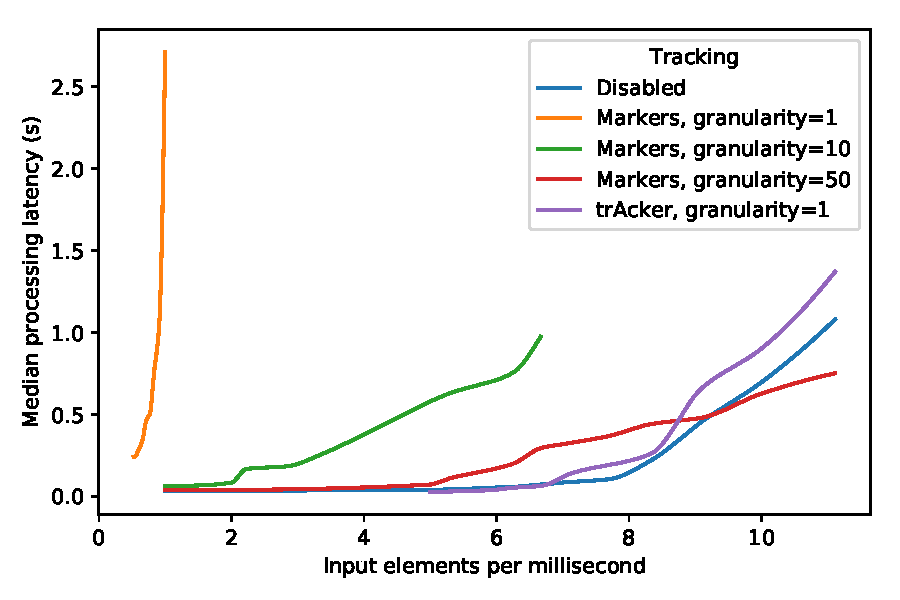
\includegraphics[width=0.99\textwidth]{pics/throughput_overhead_50.pdf}
            \caption{Overhead on an SPE throughput}
            \label{throughput_overhead}
    \end{subfigure}
    \hspace{5mm}
    \begin{subfigure}[b]{0.30\textwidth}
            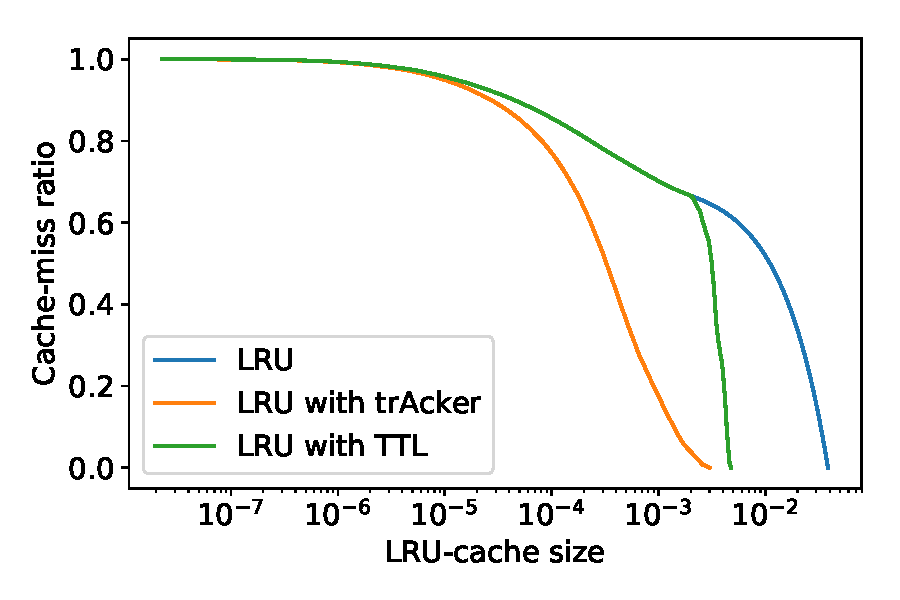
\includegraphics[width=0.99\textwidth]{pics/dgc_lru_depth_search.pdf}
            \caption{State smart cache scenario}
            \label{fig:dgc_lru_depth_search}
    \end{subfigure}
    \caption{Real-world scenarios and maximum throughput}
    \label{various_experiments}
\end{figure*}

As we mentioned above, an important application of substream tracking mechanisms is state snapshotting. Typically, state snapshotting is implemented as follows: a streaming system divides input records into the contiguous substreams called epochs. When an operator entirely processes all items from a particular epoch, it blocks all inputs and persistently saves its local state. Each operator receives the termination event for an epoch and starts to save its state independently from other operators. Flink~\cite{Carbone:2017:SMA:3137765.3137777}, Storm~\cite{apache:storm:state}, IBM Streams~\cite{jacques2016consistent}, and Heron~\cite{Kulkarni:2015:THS:2723372.2742788} implement this state snapshotting scheme. All these systems use punctuation-based techniques to provide notifications for operators.

Punctuations mechanism can imply latency overhead on this protocol. The overhead is caused by blocking an operator after the first punctuation is received until the operator receives punctuations from all inputs. This behavior is known as {\em punctuations alignment} issue~\cite{Carbone:2017:SMA:3137765.3137777}. In the case of \tracker , an operator must buffer elements from the next epoch until the NEOSS for the previous epoch is received.

Figure~\ref{snapshot_spikes} demonstrates SPE latency spikes during state snapshotting for punctuations and \tracker, depending on the persistent save duration. In general, \tracker\ provides 50-120 milliseconds fewer latency spikes. This difference can be significant for latency-conscious applications~\cite{zhang2017sub}. The low notification latency explains this difference, as we demonstrated in Section~\ref{absolute-latency}. 

% Low notification latency leads to a smaller number of elements that need to wait (be buffered), as it is shown in Figure~\ref{snapshot_buffered}. The smaller number of buffered records causes lower buffering duration that implies lower spikes in general. Note that the vast difference in the number of buffered elements does not necessarily imply the vast difference in total buffering duration because most buffered elements wait for a tiny amount of time. This experiment indicates that \tracker\ can provide better results for a common problem that is traditionally solved using punctuations.

\subsection{End-to-end throughput}
In this experiment our goal is to find how the substream management influence maximum throughput of an SPE. We measure the median latency of RR-30 workload using cluster of 20 nodes, depending on the input rate (input elements per millisecond). The growth of median latency indicates system overloading. Input rate that corresponds to the point where latency starts to grow indicates a {\em sustainable throughput}~\cite{karimov2018benchmarking}.

Figure~\ref{throughput_overhead} shows that system without tracking at all starts to be overloaded at $\sim 9K$ requests (items) per second input rate. The system with the finest-grained centralized \tracker\ setup sustains $\sim 7K$ RPS throughput. Overloading with the punctuations-based approach depends on the granularity of tracking: the finest-grained setup does not sustain even $1K$ RPS, while the setup with the granularity of 10 has $\sim 2K$ RPS throughput. Punctuations achieve similar to centralized \tracker\ throughput ($\sim 5K$ RPS) only when they are injected once per 50 input elements.

This experiment shows that punctuations significantly bound throughput of regular processing within the fine-grained setups. It is explained by the heavy extra network traffic that we demonstrated in the Section~\ref{exp_network_traffic}. Note that this additional traffic goes through the same network channels as ordinary data items to ensure that punctuations do not overtake ordinary records. On the other hand, \tracker\ provides less additional system load due to lower extra network usage and the exploiting of additional network channels.

% \begin{figure}[htbp]
%   \centering
%   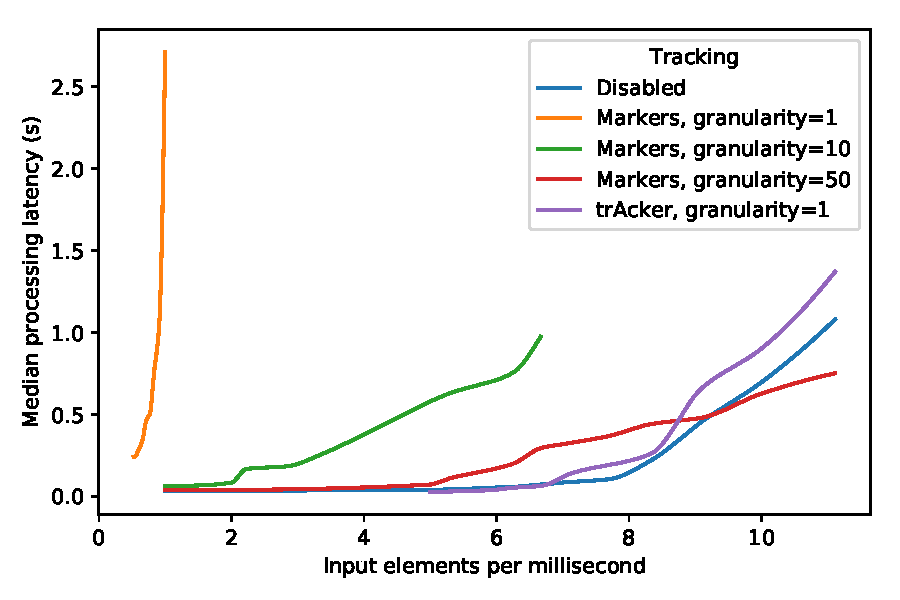
\includegraphics[width=0.40\textwidth]{pics/throughput_overhead_50.pdf}
%   \caption{Tracking overhead on a processing throughput}
%   \label{throughput_overhead}
% \end{figure}

\subsection{Substream management for cyclic graphs}
% \begin{figure}[htbp]
%   \centering
%   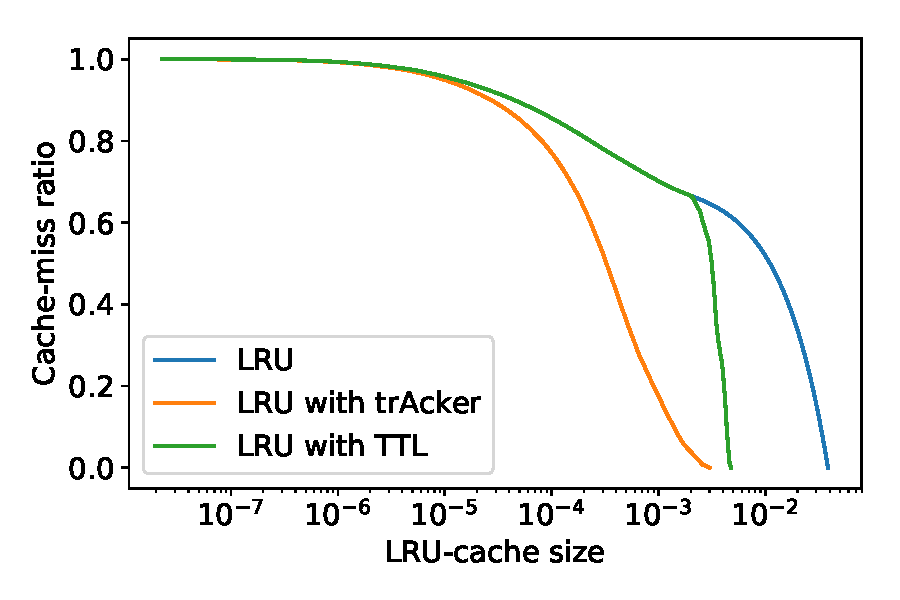
\includegraphics[width=0.40\textwidth]{pics/dgc_lru_depth_search.pdf}
%   \caption{Cache-miss ratio with the growth of share of unique keys in the system cache.}
%   \label{fig:dgc_lru_depth_search}
% \end{figure}

One more practical application of substream tracking is in-memory state optimization. In practice, we often use either short-life keys such as session-id, cart-id, or a subset of a wide variety of keys, such as users of social networks. The state associated with such keys should be removed from the memory once the key becomes obsolete. We refer to this task as \textit{distributed garbage collection}.

Substream management can be used to solve this task because we can consider elements bearing a specific key as a substream. In this experiment, we use a \tracker\ for \textit{distributed garbage collection} and compare this approach to more widespread caching techniques.

In the experimental setting, we solve a depth search problem for a graph of Twitter users. This task is relevant for social recommendation systems and requires both scalability and freshness of the results due to the dynamic nature of the graph and the number of nodes. An SPE is a suitable candidate host for such a solution due to the low latency (freshness) requirement. 

Within this model, the user is the key, and the set of her subscribers is the state associated with the key. A stream of queries of user neighborhoods is issued to the system. A resulting set of unique users is expected in return. The execution graph for the depth search problem is cyclic, so \tracker\ suits this task. 

We compare \textit{distributed garbage collection} approach with LRU caching for this task. The keys are removed from the hot set as soon as none of the currently processed messages contain a reference for it. We used a ratio of cache-misses during processing as a measure of the effectiveness of the memory management mechanism. 

In this experiment, we used 4 nodes and fixed the request per second rate to 20. In the Fig.~\ref{fig:dgc_lru_depth_search} results of this experiment are presented. With the growth of the allocated memory cache becomes effective, though the difference between 
\textit{distributed garbage collection} and LRU (with or without optimal TTL) counts in order of magnitude. We believe that this type of task needs to be resolved with GC instead of caching.